\section{Logistická regrese}\label{sec:ai-logisticka-regrese}

Při binární klasifikaci používáme třídy \(0\) a~\(1\). Přímé použití lineární regrese je problematické, protože funkce \(ax+b\) může nabývat libovolných reálných hodnot a~čtvercová chyba není přizpůsobena vyhodnocování jistoty klasifikační odpovědi. Logistická regrese proto lineární skóre převádí do intervalu \((0,1)\).

\begin{definition}\label{def:ai-sigmoida}
    \emph{Logistická funkce} neboli \emph{sigmoida} je funkce
    \[
        \sigma(z)
        =
        \frac{1}{1+e^{-z}},
        \qquad z\in\R.
    \]
\end{definition}

Funkce je rostoucí, platí \(\sigma(0)=0{,}5\) a~její hodnoty se pro velmi záporná, respektive velmi kladná \(z\), blíží \(0\), respektive \(1\).

\begin{figure}[ht]
    \centering
    \begin{tikzpicture}
    \begin{axis}[
        width=11cm,height=6cm,
        xmin=-6,xmax=6,ymin=0,ymax=1.05,
        axis lines=middle,xlabel={$z$},ylabel={$\sigma(z)$},
        xtick={0},ytick={0,0.5,1},
        yticklabels={$0$,$0{,}5$,$1$},
        label style={font=\normalsize},
        tick label style={font=\normalsize},
        every node/.style={font=\normalsize},
        clip=false
    ]
        \addplot[blue!75!black,very thick,domain=-6:6,samples=100]
            {1/(1+exp(-x))};
        \addplot[gray,dashed,domain=-6:6]{0.5};
    \end{axis}
\end{tikzpicture}

    \caption{Logistická funkce převádí reálné skóre do intervalu \((0,1)\).}
    \label{fig:ai-sigmoida}
\end{figure}

Pro jeden vstupní statistický soubor
\[
    \mathbf{X}=(x_1,\ldots,x_n)
\]
logistický model nejprve vypočítá lineární skóre \(z_i=ax_i+b\) a~potom
\[
    \hat p_i
    =
    \sigma(z_i)
    =
    \frac{1}{1+e^{-(ax_i+b)}}.
\]
Statistický soubor výstupů označíme
\[
    \hat{\mathbf{P}}
    =
    (\hat p_1,\ldots,\hat p_n).
\]
Hodnotu \(\hat p_i\) chápeme jako míru podpory modelu pro třídu \(1\).

Pro rozhodovací práh \(t\in(0,1)\) definujeme
\[
    h^{(t)}(x)
    =
    \begin{cases}
        1, & \hat p(x)\geqslant t,\\
        0, & \hat p(x)<t.
    \end{cases}
\]
Protože je sigmoida rostoucí,
\[
    \hat p(x)\geqslant t
    \quad\Longleftrightarrow\quad
    ax+b\geqslant
    \ln\left(\frac{t}{1-t}\right).
\]
Pro obvyklý práh \(t=0{,}5\) rozhoduje znaménko výrazu \(ax+b\).

\subsection{Křížová entropie}

\begin{definition}\label{def:ai-bce}
    Pro skutečnou třídu \(y_i\in\set{0,1}\) a~výstup
    \(\hat p_i\in(0,1)\) definujeme \emph{binární křížovou entropii}
    \[
        \ell(y_i,\hat p_i)
        =
        -
        \left(
            y_i\ln\hat p_i
            +(1-y_i)\ln(1-\hat p_i)
        \right).
    \]
    Průměrná křížová entropie na celém souboru je
    \[
        L(\mathbf{Y},\hat{\mathbf{P}})
        =
        \frac1n\sum_{i=1}^{n}\ell(y_i,\hat p_i).
    \]
\end{definition}

Je-li \(y_i=1\), ztráta má tvar \(-\ln\hat p_i\); je-li \(y_i=0\), má tvar \(-\ln(1-\hat p_i)\). Správná a~jistá předpověď má malou ztrátu, zatímco jistá chybná předpověď je potrestána velmi vysokou hodnotou.

Parametry logistické regrese hledáme tak, aby
\[
    (a^\ast,b^\ast)
    =
    \argmin_{(a,b)\in\R^2}L(a,b),
\]
kde
\[
    L(a,b)
    =
    -\frac1n\sum_{i=1}^{n}
    \left(
        y_i\ln\hat p_i(a,b)
        +(1-y_i)\ln(1-\hat p_i(a,b))
    \right).
\]

\subsection{Odbočka: co vyjadřuje derivace}\label{subsec:ai-derivace}

K~hledání minima potřebujeme vědět, jak se hodnota funkce změní při malé změně jejího vstupu. Pro funkci jedné proměnné \(g\) porovnáváme hodnoty \(g(c)\) a~\(g(c+h)\). Podíl
\[
    \frac{g(c+h)-g(c)}{h}
\]
je směrnice sečny vedené dvěma blízkými body grafu. Necháme-li nenulové \(h\) přibližovat k~nule a~směrnice se ustálí, získáme \emph{derivaci} \(g'(c)\). Derivace tedy popisuje okamžitý směr a~rychlost změny:
\begin{itemize}
    \item \(g'(c)>0\): funkce v~okolí \(c\) roste;
    \item \(g'(c)<0\): funkce v~okolí \(c\) klesá;
    \item \(g'(c)=0\): graf má v~daném bodě vodorovnou tečnu; může zde ležet minimum nebo maximum.
\end{itemize}

\begin{figure}[ht]
    \centering
    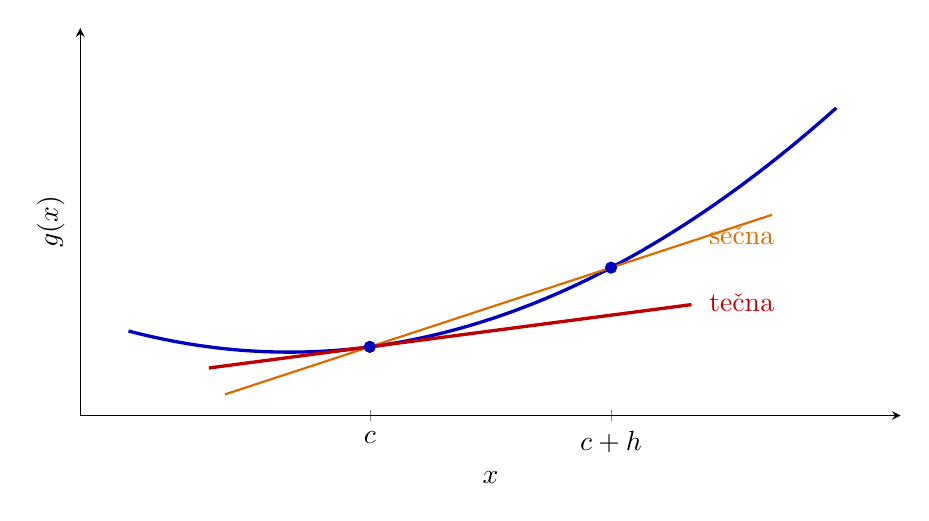
\begin{tikzpicture}
    \begin{axis}[
        width=12cm,height=6.5cm,
        xmin=-0.3,xmax=4.8,ymin=-0.3,ymax=5.2,
        axis lines=left,xlabel={$x$},ylabel={$g(x)$},
        xtick={1.5,3},xticklabels={$c$,$c+h$},
        ytick=\empty,
        label style={font=\normalsize},
        tick label style={font=\normalsize},
        every node/.style={font=\normalsize},
        clip=false
    ]
        \addplot[blue!75!black,very thick,domain=0:4.4,samples=100]
            {0.3*(x-1)^2+0.6};
        % Sečna prochází body (c,g(c))=(1.5,0.675) a
        % (c+h,g(c+h))=(3,1.8); její směrnice je 0.75.
        \addplot[orange!85!black,thick,domain=0.6:4]
            {0.75*x-0.45};
        % Derivace g'(x)=0.6(x-1), takže tečna v c=1.5 má
        % směrnici 0.3 a rovnici y=0.3x+0.225.
        \addplot[red!75!black,very thick,domain=0.5:3.5]
            {0.3*x+0.225};
        \addplot[only marks,mark=*,blue!75!black]
            coordinates{(1.5,0.675)(3,1.8)};
        \node[orange!85!black,anchor=west] at (axis cs:3.55,2.25){sečna};
        \node[red!75!black,anchor=west] at (axis cs:3.55,1.30){tečna};
    \end{axis}
\end{tikzpicture}

    \caption{Sečna se při zmenšování \(h\) blíží tečně; její směrnice je derivací.}
    \label{fig:ai-derivace}
\end{figure}

Závisí-li ztráta \(L(a,b)\) na dvou parametrech, můžeme měnit vždy jen jeden z~nich. Symboly
\[
    \frac{\partial L}{\partial a},
    \qquad
    \frac{\partial L}{\partial b}
\]
označují derivace podle \(a\), respektive podle \(b\), při pevném druhém parametru. Vektor
\[
    \nabla L(a,b)
    =
    \left(
        \frac{\partial L}{\partial a},
        \frac{\partial L}{\partial b}
    \right)
\]
nazýváme \emph{gradient}. Ukazuje směrem nejrychlejšího růstu ztráty, a~proto se při minimalizaci pohybujeme opačným směrem.

\subsection{Gradientní sestup}

Pro logistickou regresi lze odvodit
\[
    \frac{\partial L}{\partial a}
    =
    \frac1n\sum_{i=1}^{n}
    (\hat p_i-y_i)x_i,
    \qquad
    \frac{\partial L}{\partial b}
    =
    \frac1n\sum_{i=1}^{n}
    (\hat p_i-y_i).
\]
Při rychlosti učení \(\eta>0\) opakujeme aktualizace
\[
    a
    \gets
    a-\eta\frac{\partial L}{\partial a},
    \qquad
    b
    \gets
    b-\eta\frac{\partial L}{\partial b}.
\]

\begin{figure}[ht]
    \centering
    \begin{tikzpicture}
    \begin{axis}[
        width=12cm,height=6.2cm,
        xmin=-4,xmax=6,ymin=0,ymax=9,
        axis lines=left,xlabel={parametr},ylabel={\(L\)},
        xtick=\empty,ytick=\empty,
        label style={font=\normalsize},
        every node/.style={font=\normalsize},
        clip=false
    ]
        \addplot[blue!75!black,very thick,domain=-3.8:5.8,samples=100]
            {0.3*(x-1)^2+0.5};
        \foreach \x in {5,3.4,2.3,1.6,1.2}{
            \pgfmathsetmacro{\y}{0.3*(\x-1)^2+0.5}
            \addplot[only marks,mark=*,mark size=2.5pt,red!75!black]
                coordinates{(\x,\y)};
        }
        \draw[diredge,red!75!black] (axis cs:5,5.3)--(axis cs:3.4,2.228);
        \draw[diredge,red!75!black] (axis cs:3.4,2.228)--(axis cs:2.3,1.007);
        \draw[diredge,red!75!black] (axis cs:2.3,1.007)--(axis cs:1.6,0.608);
        \draw[diredge,red!75!black] (axis cs:1.6,0.608)--(axis cs:1.2,0.512);
        \node[above] at (axis cs:1,0.72){minimum};
    \end{axis}
\end{tikzpicture}

    \caption{Gradientní sestup postupně snižuje hodnotu ztrátové funkce.}
    \label{fig:ai-gradientni-sestup}
\end{figure}

Příliš malá \(\eta\) vede k~pomalému postupu. Příliš velká hodnota může minimum přeskakovat nebo výpočet rozkmitat. Zastavujeme například po pevném počtu iterací nebo ve chvíli, kdy se ztráta a~parametry mění už jen nepatrně.

Jedna iterace využije všechny trénovací objekty k~výpočtu průměrného gradientu. Takové variantě říkáme \emph{dávkový gradientní sestup}. U~velkých souborů lze gradient odhadovat z~menších náhodných dávek; aktualizace jsou potom levnější, ale jejich směr více kolísá.

\begin{algorithm}
    \caption{\textsc{logistic-regression}}
    \label{alg:ai-logistic-regression}
    \KwIn{Soubory \(\mathbf{X}=(x_1,\ldots,x_n)\), \(\mathbf{Y}=(y_1,\ldots,y_n)\), rychlost učení \(\eta>0\) a~počet iterací \(T\)}
    \(a\gets0\), \(b\gets0\)\\
    \For{\(r\gets1,2,\ldots,T\)}{
        \For{\(i\gets1,2,\ldots,n\)}{
            \(\displaystyle\hat p_i\gets\frac{1}{1+e^{-(ax_i+b)}}\)
        }
        \(\displaystyle g_a\gets\frac1n\sum_{i=1}^{n}(\hat p_i-y_i)x_i\)\\
        \(\displaystyle g_b\gets\frac1n\sum_{i=1}^{n}(\hat p_i-y_i)\)\\
        \(a\gets a-\eta g_a\), \(b\gets b-\eta g_b\)
    }
    \KwOut{Parametry \(a,b\) a~skóre \(\hat p(x)=\sigma(ax+b)\)}
\end{algorithm}

\subsection{Implementace v~Pythonu}

Program~\ref{lst:ai-logistic-regression} používá přesně uvedené dva gradienty. Metoda \texttt{fit} opakovaně vypočítá všechny hodnoty \(\hat p_i\) a~upraví parametry \(a,b\); metoda \texttt{predict} převede výstupy na třídy pomocí zvoleného prahu.

Funkce \texttt{sigmoid} je zapsána ve dvou algebraicky ekvivalentních větvích. Pro záporné \(z\) používá výraz s~\(e^z\), aby při velmi záporném vstupu nemusela počítat obrovskou hodnotu \(e^{-z}\). Jde o~technickou úpravu numerické stability, nikoli o~změnu matematického modelu.

\lstinputlisting[
    caption={Logistická regrese pro jeden vstupní statistický znak.},
    label={lst:ai-logistic-regression}
]{07-ai/code/logistic_regression.py}

Ukázka používá jeden vstupní znak, aby byl vztah mezi parametry a~rozhodovací hranicí dobře vidět. Pro více znaků nahradíme \(ax+b\) výrazem \(\sum_{j=1}^{p}w_jx_j+\theta\) a~pro každou váhu \(w_j\) počítáme vlastní složku gradientu; princip pseudokódu zůstává stejný.
